\documentclass[10pt]{article}
\usepackage{tikz}
\usetikzlibrary{shapes.misc}
\usepackage[margin=0cm]{geometry}
\pagestyle{empty}
\tikzstyle{every node}=[cross out, draw, red]

\begin{document}

\vspace*{\fill}
\begin{center}
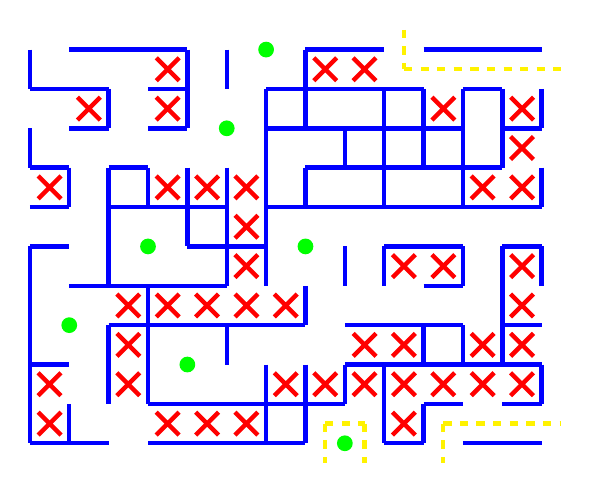
\begin{tikzpicture}[x=0.5cm, y=-0.5cm, ultra thick, blue]
% Walls
    \draw (1,0) -- (4,0);
    \draw (7,0) -- (9,0);
    \draw (10,0) -- (13,0);
    \draw (0,1) -- (2,1);
    \draw (3,1) -- (4,1);
    \draw (6,1) -- (10,1);
    \draw (11,1) -- (12,1);
    \draw (1,2) -- (2,2);
    \draw (3,2) -- (4,2);
    \draw (6,2) -- (11,2);
    \draw (12,2) -- (13,2);
    \draw (0,3) -- (1,3);
    \draw (2,3) -- (3,3);
    \draw (7,3) -- (12,3);
    \draw (0,4) -- (1,4);
    \draw (2,4) -- (5,4);
    \draw (6,4) -- (13,4);
    \draw (0,5) -- (1,5);
    \draw (4,5) -- (6,5);
    \draw (9,5) -- (11,5);
    \draw (12,5) -- (13,5);
    \draw (1,6) -- (5,6);
    \draw (10,6) -- (11,6);
    \draw (2,7) -- (7,7);
    \draw (8,7) -- (11,7);
    \draw (12,7) -- (13,7);
    \draw (0,8) -- (1,8);
    \draw (8,8) -- (13,8);
    \draw (3,9) -- (8,9);
    \draw (10,9) -- (11,9);
    \draw (12,9) -- (13,9);
    \draw (0,10) -- (2,10);
    \draw (3,10) -- (7,10);
    \draw (9,10) -- (10,10);
    \draw (11,10) -- (13,10);
    \draw (0,0) -- (0,1);
    \draw (0,2) -- (0,3);
    \draw (0,5) -- (0,10);
    \draw (1,3) -- (1,4);
    \draw (1,9) -- (1,10);
    \draw (2,1) -- (2,2);
    \draw (2,3) -- (2,6);
    \draw (2,7) -- (2,9);
    \draw (3,3) -- (3,4);
    \draw (3,6) -- (3,9);
    \draw (4,0) -- (4,2);
    \draw (4,3) -- (4,5);
    \draw (5,0) -- (5,1);
    \draw (5,3) -- (5,6);
    \draw (5,7) -- (5,8);
    \draw (6,1) -- (6,6);
    \draw (6,8) -- (6,10);
    \draw (7,0) -- (7,2);
    \draw (7,3) -- (7,4);
    \draw (7,6) -- (7,7);
    \draw (7,8) -- (7,10);
    \draw (8,2) -- (8,3);
    \draw (8,5) -- (8,6);
    \draw (8,8) -- (8,9);
    \draw (9,1) -- (9,4);
    \draw (9,5) -- (9,6);
    \draw (9,8) -- (9,10);
    \draw (10,1) -- (10,3);
    \draw (10,7) -- (10,8);
    \draw (10,9) -- (10,10);
    \draw (11,1) -- (11,4);
    \draw (11,5) -- (11,6);
    \draw (11,7) -- (11,8);
    \draw (12,1) -- (12,3);
    \draw (12,5) -- (12,8);
    \draw (13,1) -- (13,2);
    \draw (13,3) -- (13,4);
    \draw (13,5) -- (13,6);
    \draw (13,8) -- (13,9);
% Pillars
    \fill[green] (6,0) circle(0.2);
    \fill[green] (5,2) circle(0.2);
    \fill[green] (3,5) circle(0.2);
    \fill[green] (7,5) circle(0.2);
    \fill[green] (1,7) circle(0.2);
    \fill[green] (4,8) circle(0.2);
    \fill[green] (8,10) circle(0.2);
% Inner points in accessible cul-de-sacs
    \node at (3.5,0.5) {};
    \node at (7.5,0.5) {};
    \node at (8.5,0.5) {};
    \node at (1.5,1.5) {};
    \node at (3.5,1.5) {};
    \node at (10.5,1.5) {};
    \node at (12.5,1.5) {};
    \node at (12.5,2.5) {};
    \node at (0.5,3.5) {};
    \node at (3.5,3.5) {};
    \node at (4.5,3.5) {};
    \node at (5.5,3.5) {};
    \node at (11.5,3.5) {};
    \node at (12.5,3.5) {};
    \node at (5.5,4.5) {};
    \node at (5.5,5.5) {};
    \node at (9.5,5.5) {};
    \node at (10.5,5.5) {};
    \node at (12.5,5.5) {};
    \node at (2.5,6.5) {};
    \node at (3.5,6.5) {};
    \node at (4.5,6.5) {};
    \node at (5.5,6.5) {};
    \node at (6.5,6.5) {};
    \node at (12.5,6.5) {};
    \node at (2.5,7.5) {};
    \node at (8.5,7.5) {};
    \node at (9.5,7.5) {};
    \node at (11.5,7.5) {};
    \node at (12.5,7.5) {};
    \node at (0.5,8.5) {};
    \node at (2.5,8.5) {};
    \node at (6.5,8.5) {};
    \node at (7.5,8.5) {};
    \node at (8.5,8.5) {};
    \node at (9.5,8.5) {};
    \node at (10.5,8.5) {};
    \node at (11.5,8.5) {};
    \node at (12.5,8.5) {};
    \node at (0.5,9.5) {};
    \node at (3.5,9.5) {};
    \node at (4.5,9.5) {};
    \node at (5.5,9.5) {};
    \node at (9.5,9.5) {};
% Entry-exit paths without intersections
    \draw[dashed, yellow] (9.5,0.5) -- (13.5,0.5);
    \draw[dashed, yellow] (7.5,9.5) -- (8.5,9.5);
    \draw[dashed, yellow] (10.5,9.5) -- (13.5,9.5);
    \draw[dashed, yellow] (7.5,9.5) -- (7.5,10.5);
    \draw[dashed, yellow] (8.5,9.5) -- (8.5,10.5);
    \draw[dashed, yellow] (9.5,-0.5) -- (9.5,0.5);
    \draw[dashed, yellow] (10.5,9.5) -- (10.5,10.5);
\end{tikzpicture}
\end{center}
\vspace*{\fill}

\end{document}
